\chapter{Analisi dei requisiti}
\label{cap:analisi-requisiti}

\intro{Il seguente capitolo assume la funzione di illustrare i casi d'uso e i requisiti raccolti nella fase di analisi del progetto commissionato.}

\setlength{\parskip}{3ex}

\section{Casi d'uso}
Per poter capire e studiare a fondo tutte le funzionalità che devono essere messe a disposizione dell'utente che utilizza l'applicativo da sviluppare, sono stati realizzati i relativi diagrammi dei casi d'uso di tipo {\hyperref[sec:uml-definition]{UML}}\glsfirstoccur. Tali diagrammi sono risultati fondamentali per individuare correttamente tutti i requisiti del sistema in questione.

\setlength{\parskip}{3ex}

\noindent Ciascun caso d'uso è costituito da:
\begin{itemize}
\item attore primario;
\item precondizione;
\item postcondizione;
\item scenario principale;
\item generalizzazioni (qualora fossero presenti);
\item estensioni (qualora fossero presenti).
\end{itemize}

\setlength{\parskip}{3ex}

\noindent I casi d'uso identificati dalla sigla "UCE" rappresentano un caso d'uso d'errore.
L'unico attore coinvolto e identificato come \textit{Utente autenticato} corrisponde ad un qualunque dipendente dell'area commerciale di CWBI, al quale sono stati assegnati i permessi necessari a svolgere le operazioni di seguito riportate.  

\pagebreak

\subsection{UC0: Menu}
\begin{figure}[!h]
\centering
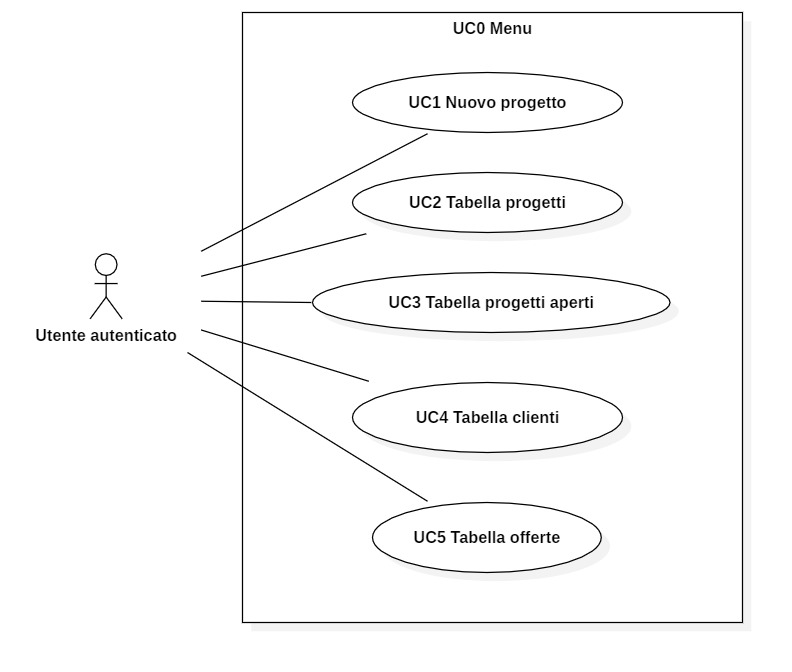
\includegraphics[width=300px]{../images/UC/.jpeg/UC0-menu.jpg}
\caption{UC0: Menu}
\end{figure}

\begin{itemize}
\item \textbf{Attore primario}: Utente autenticato.
\item \textbf{Precondizione}: L'attore ha accesso al modulo \textit{Campaign} della webapp CW GEST.
\item \textbf{Postcondizione}: Il sistema è pronto all'uso.
\item \textbf{Scenario principale}: 
\begin{enumerate}
\item L'attore crea un nuovo progetto [UC1].
\item L'attore accede alla tabella dei progetti [UC2].
\item L'attore accede alla tabella dei progetti aperti [UC3].
\item L'attore accede alla tabella dei clienti [UC4].
\item L'attore accede alla tabella delle offerte [UC5].
\end{enumerate}
\end{itemize}

\pagebreak

\subsection{UC1: Crea-Modifica progetto}
\begin{figure}[!h]
\centering
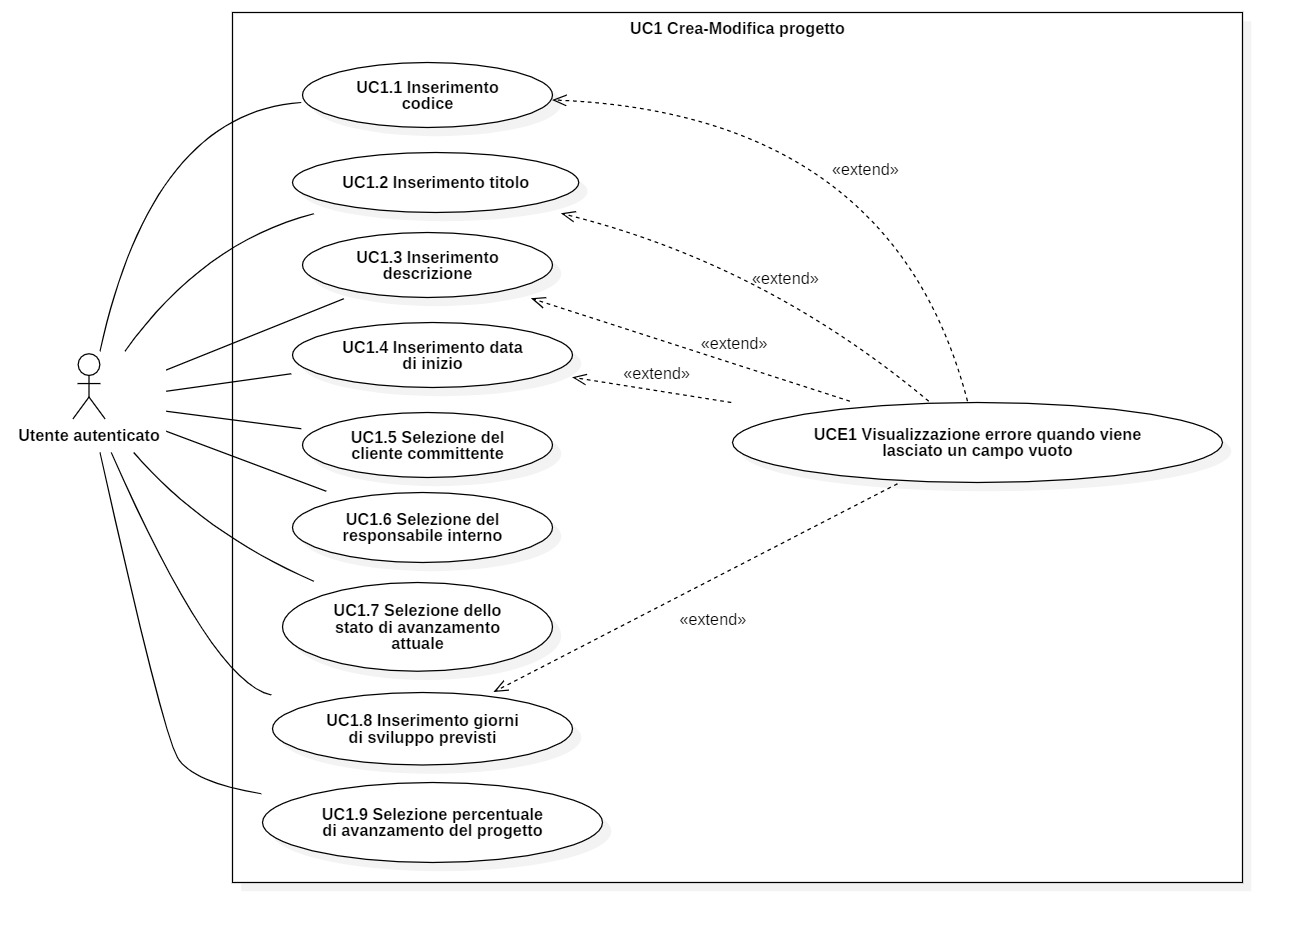
\includegraphics[width=400px]{../images/UC/.jpeg/UC1-nuovoModificaProgetto.jpg}
\caption{UC1: Crea-Modifica progetto}
\end{figure}

\begin{itemize}
\item \textbf{Attore primario}: Utente autenticato.
\item \textbf{Precondizione}: L'attore ha selezionato: 
\begin{itemize}
\item l'opzione \textit{nuovo progetto} dal menu;
\item l'opzione \textit{modifica} dal dettaglio di un progetto
\end{itemize}
\item \textbf{Postcondizione}: L'attore ha creato/modificato un progetto.
\item \textbf{Scenario principale}: 
\begin{enumerate}
\item L'attore inserisce/modifica il codice del progetto [UC1.1].
\item L'attore inserisce/modifica il titolo del progetto [UC1.2].
\item L'attore inserisce/modifica la descrizione del progetto [UC1.3].
\item L'attore inserisce/modifica la data di inizio del progetto [UC1.4].
\item L'attore seleziona/modifica il cliente committente [UC1.5].
\item L'attore seleziona/modifica il responsabile interno assegnato al progetto [UC1.6].
\item L'attore seleziona/modifica lo stato di avanzamento attuale delle attività [UC1.7].
\item L'attore inserisce/modifica i giorni di sviluppo previsti [UC1.8].
\item L'attore seleziona/modifica la percentuale di avanzamento delle attività di progetto [UC1.9].
\end{enumerate}
\item \textbf{Estensioni}: 
\begin{itemize}
\item L'attore visualizza un messaggio di errore quando viene lasciato un campo vuoto [UCE1].
\end{itemize} 
\end{itemize}

\pagebreak

\subsection{UC2: Tabella progetti}
\begin{figure}[!h]
\centering
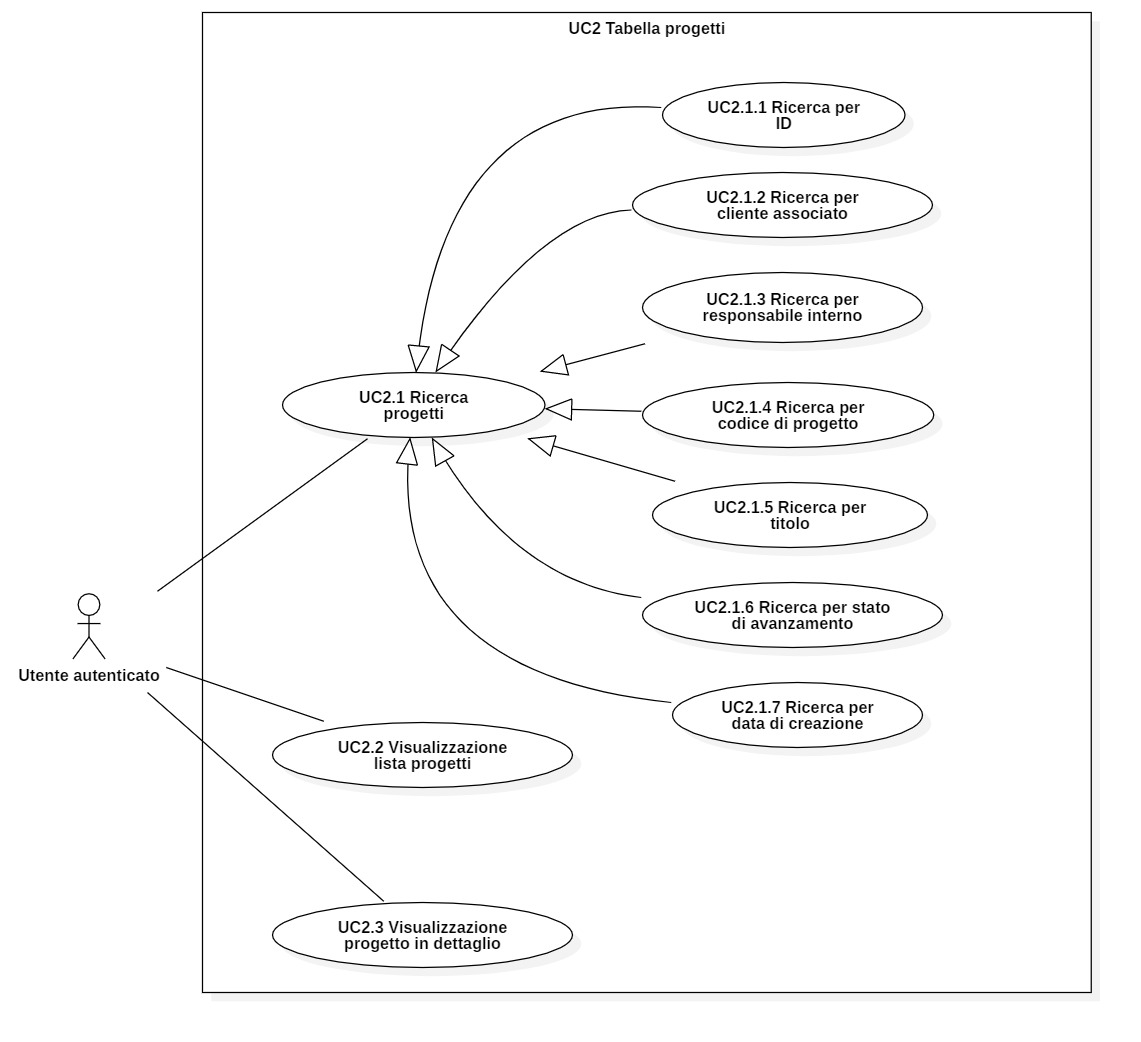
\includegraphics[width=400px]{../images/UC/.jpeg/UC2.0-tabellaProgetti.jpg}
\caption{UC2: Tabella progetti}
\end{figure}

\begin{itemize}
\item \textbf{Attore primario}: Utente autenticato.
\item \textbf{Precondizione}: L'attore ha selezionato l'opzione \textit{tabella progetti} dal menu.
\item \textbf{Postcondizione}: L'attore ha accesso alla tabella dei progetti.
\item \textbf{Scenario principale}: 
\begin{enumerate}
\item L'attore cerca uno o più progetti tramite la funzionalità di ricerca [UC2.1].
\item L'attore visualizza la lista completa dei progetti presenti nel sistema [UC2.2].
\item L'attore visualizza un progetto nel dettaglio [UC2.3].
\end{enumerate}
\item \textbf{Generalizzazioni}:
\begin{enumerate}
\item L'attore ricerca un progetto per ID [UC2.1.1].
\item L'attore ricerca un progetto per uno specifico cliente associato [UC2.1.2].
\item L'attore ricerca un progetto per responsabile interno [UC2.1.3].
\item L'attore ricerca un progetto per codice [UC2.1.4].
\item L'attore ricerca un progetto per titolo [UC2.1.5].
\item L'attore ricerca un progetto per stato di avanzamento [UC2.1.6].
\item L'attore ricerca un progetto per data di creazione [UC2.1.7].
\end{enumerate}
\end{itemize}

\pagebreak

\subsection{UC2.2: Visualizzazione lista progetti}
\begin{figure}[!h]
\centering
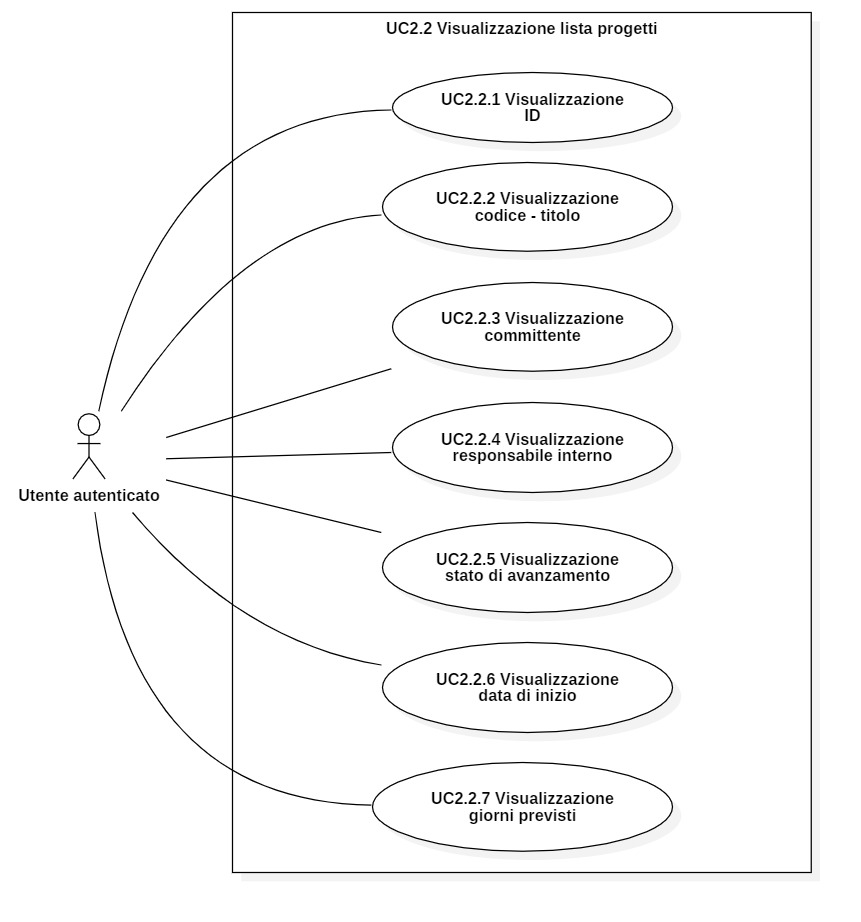
\includegraphics[width=300px]{../images/UC/.jpeg/UC2.2-visualizzazioneListaProgetti.jpg}
\caption{UC2.2: Visualizzazione lista progetti}
\end{figure}

\begin{itemize}
\item \textbf{Attore primario}: Utente autenticato.
\item \textbf{Precondizione}: L'attore ha accesso alla tabella dei progetti.
\item \textbf{Postcondizione}: L'attore ha visualizzato la lista dei progetti.
\item \textbf{Scenario principale}: 
\begin{enumerate}
\item L'attore visualizza l'ID del progetto [UC2.2.1].
\item L'attore visualizza la stringa "codice - titolo" del progetto [UC2.2.2].
\item L'attore visualizza il committente del progetto [UC2.2.3].
\item L'attore visualizza il responsabile interno del progetto [UC2.2.4].
\item L'attore visualizza lo stato di avanzamento del progetto [UC2.2.5].
\item L'attore visualizza la data di inizio del progetto [UC2.2.6].
\item L'attore visualizza i giorni di sviluppo previsti del progetto [UC2.2.7].
\end{enumerate}
\end{itemize}

\pagebreak

\subsection{UC2.3: Visualizzazione progetto in dettaglio}
\begin{figure}[!h]
\centering
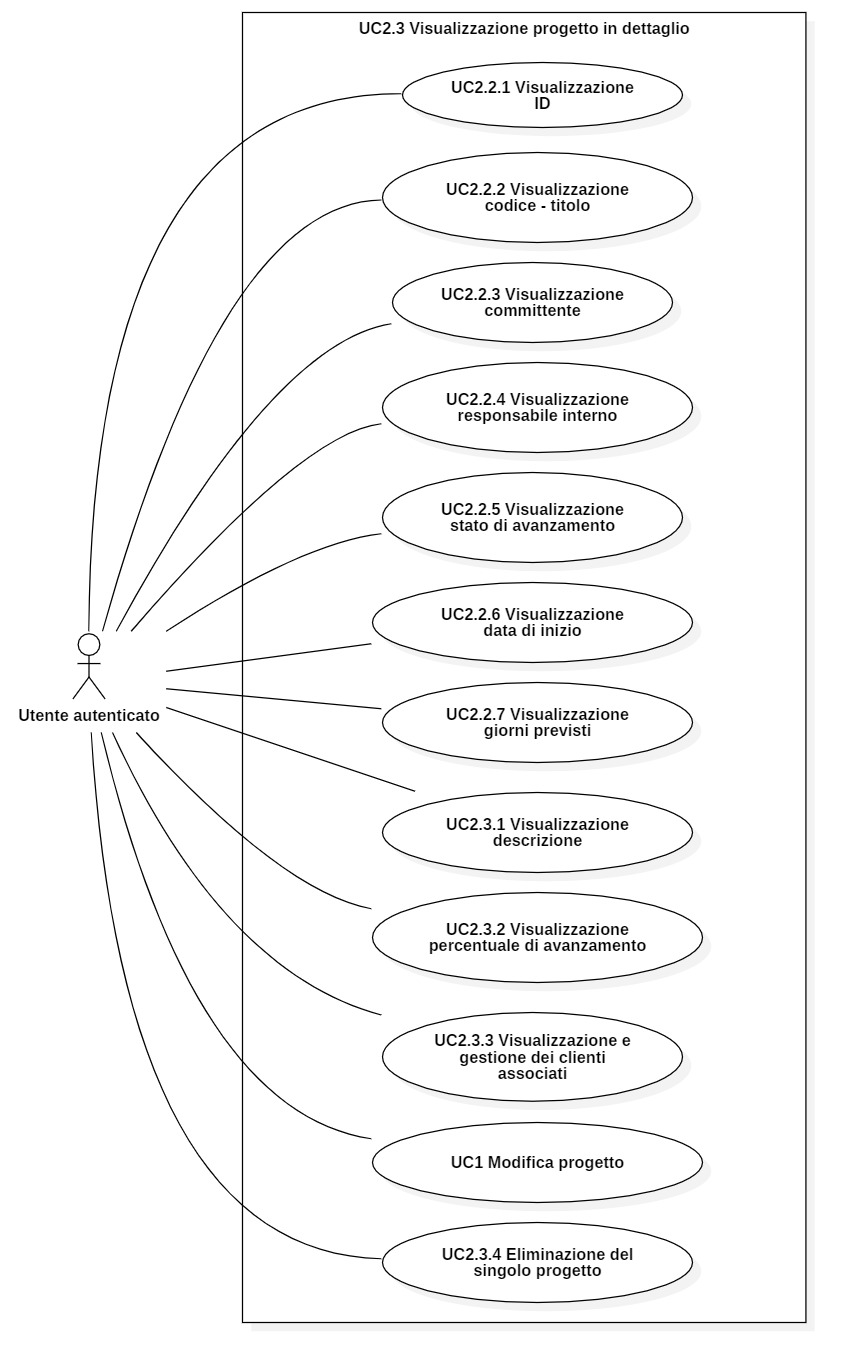
\includegraphics[width=300px]{../images/UC/.jpeg/UC2.3-visualizzazioneDettaglioProgetto.jpg}
\caption{UC2.3: Visualizzazione progetto in dettaglio}
\end{figure}

\begin{itemize}
\item \textbf{Attore primario}: Utente autenticato.
\item \textbf{Precondizione}: L'attore ha accesso alla tabella dei progetti.
\item \textbf{Postcondizione}: L'attore ha visualizzato il dettaglio di un progetto.
\item \textbf{Scenario principale}: 
\begin{enumerate}
\item L'attore visualizza l'ID del progetto [UC2.2.1].
\item L'attore visualizza la stringa "codice - titolo" del progetto [UC2.2.2].
\item L'attore visualizza il committente del progetto [UC2.2.3].
\item L'attore visualizza il responsabile interno del progetto [UC2.2.4].
\item L'attore visualizza lo stato di avanzamento del progetto [UC2.2.5].
\item L'attore visualizza la data di inizio del progetto [UC2.2.6].
\item L'attore visualizza i giorni di sviluppo previsti del progetto [UC2.2.7].
\item L'attore visualizza la descrizione del progetto [UC2.3.1].
\item L'attore visualizza la percentuale di avanzamento del progetto [UC2.3.2].
\item L'attore visualizza e gestisce i clienti associati al progetto [UC2.3.3].
\item L'attore può modificare il progetto [UC1].
\item L'attore può eliminare il progetto [UC2.3.4].
\end{enumerate}
\end{itemize}

\pagebreak

\subsection{UC3: Tabella progetti aperti}
\begin{figure}[!h]
\centering
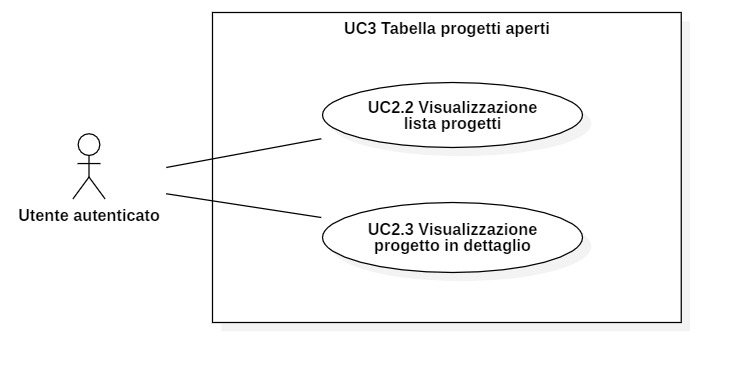
\includegraphics[width=300px]{../images/UC/.jpeg/UC3.0-tabellaProgettiAperti.jpg}
\caption{UC3: Tabella progetti aperti}
\end{figure}

\begin{itemize}
\item \textbf{Attore primario}: Utente autenticato.
\item \textbf{Precondizione}: L'attore ha selezionato l'opzione \textit{tabella progetti aperti} dal menu.
\item \textbf{Postcondizione}: L'attore ha accesso alla tabella dei progetti aperti.
\item \textbf{Scenario principale}: 
\begin{enumerate}
\item L'attore visualizza la lista dei progetti aperti presenti nel sistema [UC2.2].
\item L'attore visualizza un progetto aperto nel dettaglio [UC2.3].
\end{enumerate}
\end{itemize}

\pagebreak

\subsection{UC4: Tabella clienti}
\begin{figure}[!h]
\centering
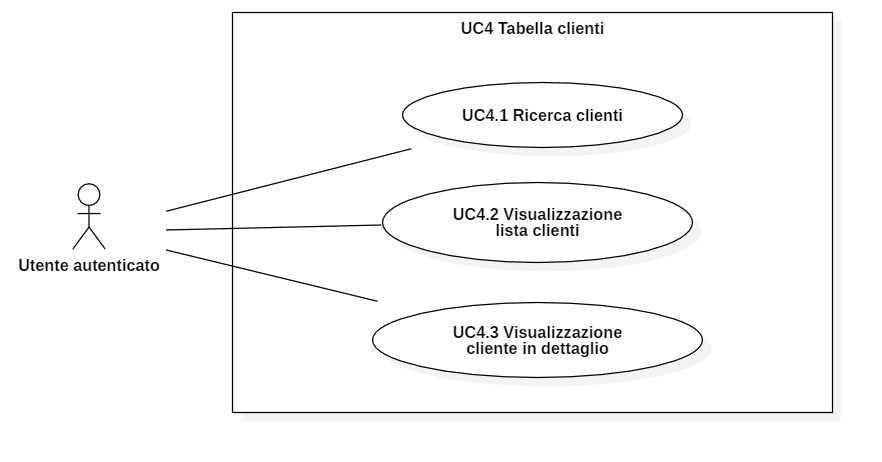
\includegraphics[width=400px]{../images/UC/.jpeg/UC4.0-tabellaClienti.jpg}
\caption{UC4: Tabella clienti}
\end{figure}

\begin{itemize}
\item \textbf{Attore primario}: Utente autenticato.
\item \textbf{Precondizione}: L'attore ha selezionato l'opzione \textit{tabella clienti} dal menu.
\item \textbf{Postcondizione}: L'attore ha accesso alla tabella dei clienti.
\item \textbf{Scenario principale}: 
\begin{enumerate}
\item L'attore cerca uno o più clienti tramite la funzionalità di ricerca [UC4.1].
\item L'attore visualizza la lista completa dei clienti presenti nel sistema [UC4.2].
\item L'attore visualizza un cliente nel dettaglio [UC4.3].
\end{enumerate}
\item \textbf{Generalizzazioni}:
\begin{enumerate}
\item L'attore ricerca un cliente per ID [UC4.1.1].
\item L'attore ricerca un cliente per codice (nominativo aziendale) [UC4.1.2].
\item L'attore ricerca un cliente per descrizione [UC4.1.3].
\end{enumerate}
\end{itemize}

\pagebreak

\subsection{UC4.2: Visualizzazione lista clienti}
\begin{figure}[!h]
\centering
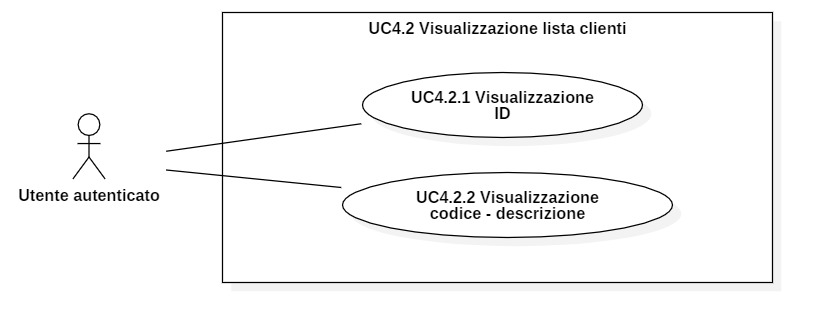
\includegraphics[width=300px]{../images/UC/.jpeg/UC4.2-visualizzazioneListaClienti.jpg}
\caption{UC4.2: Visualizzazione lista clienti}
\end{figure}

\begin{itemize}
\item \textbf{Attore primario}: Utente autenticato.
\item \textbf{Precondizione}: L'attore ha accesso alla tabella dei clienti.
\item \textbf{Postcondizione}: L'attore ha visualizzato la lista dei clienti.
\item \textbf{Scenario principale}: 
\begin{enumerate}
\item L'attore visualizza l'ID del cliente [UC4.2.1].
\item L'attore visualizza la stringa "codice - descrizione" del cliente [UC4.2.2].
\end{enumerate}
\end{itemize}

\pagebreak

\subsection{UC4.3: Visualizzazione cliente in dettaglio}
\begin{figure}[!h]
\centering
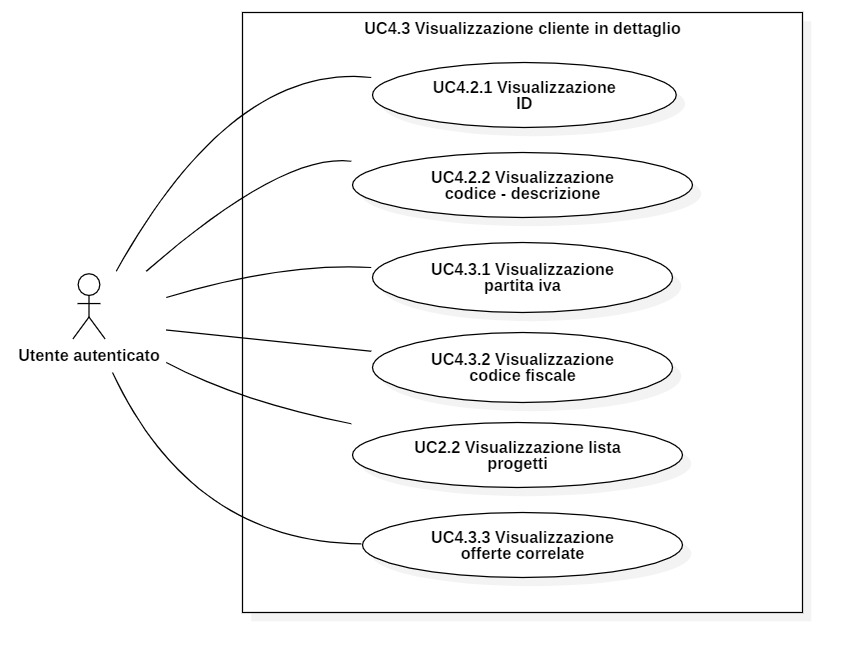
\includegraphics[width=300px]{../images/UC/.jpeg/UC4.3.0-visualizzazioneDettaglioCliente.jpg}
\caption{UC4.3: Visualizzazione cliente in dettaglio}
\end{figure}

\begin{itemize}
\item \textbf{Attore primario}: Utente autenticato.
\item \textbf{Precondizione}: L'attore ha accesso alla tabella dei clienti.
\item \textbf{Postcondizione}: L'attore ha visualizzato il dettaglio di un cliente.
\item \textbf{Scenario principale}: 
\begin{enumerate}
\item L'attore visualizza l'ID del cliente [UC4.2.1].
\item L'attore visualizza la stringa "codice - descrizione" del cliente [UC4.2.2].
\item L'attore visualizza la partita iva del cliente [UC4.3.1].
\item L'attore visualizza il codice fiscale del cliente [UC4.3.2].
\item L'attore visualizza la lista dei progetti associati al cliente [UC2.2].
\item L'attore visualizza le offerte correlate al cliente [UC4.3.3].
\end{enumerate}
\end{itemize}

\pagebreak

\subsection{UC4.3.3: Visualizzazione offerte correlate}
\begin{figure}[!h]
\centering
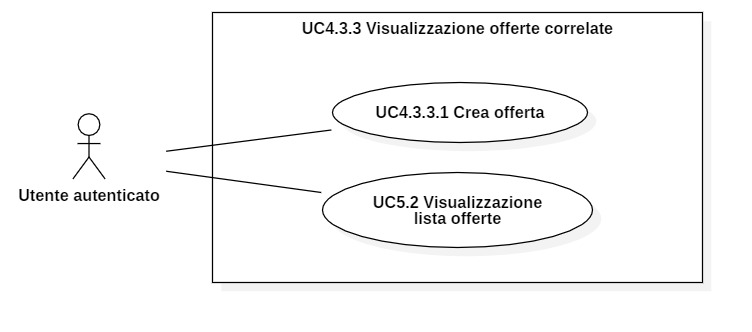
\includegraphics[width=300px]{../images/UC/.jpeg/UC4.3.3.0-visualizzazioneOfferteCorrelate.jpg}
\caption{UC4.3.3: Visualizzazione offerte correlate}
\end{figure}

\begin{itemize}
\item \textbf{Attore primario}: Utente autenticato.
\item \textbf{Precondizione}: L'attore ha visualizzato il dettaglio di un cliente.
\item \textbf{Postcondizione}: L'attore ha visualizzato le offerte correlate al cliente.
\item \textbf{Scenario principale}:
\begin{enumerate}
\item L'attore può creare una nuova offerta correlata al cliente [UC4.3.3.1].
\item L'attore visualizza la lista delle offerte del cliente [UC5.2].
\end{enumerate}
\end{itemize}

\pagebreak

\subsection{UC4.3.3.1: Crea-Modifica offerta}
\begin{figure}[!h]
\centering
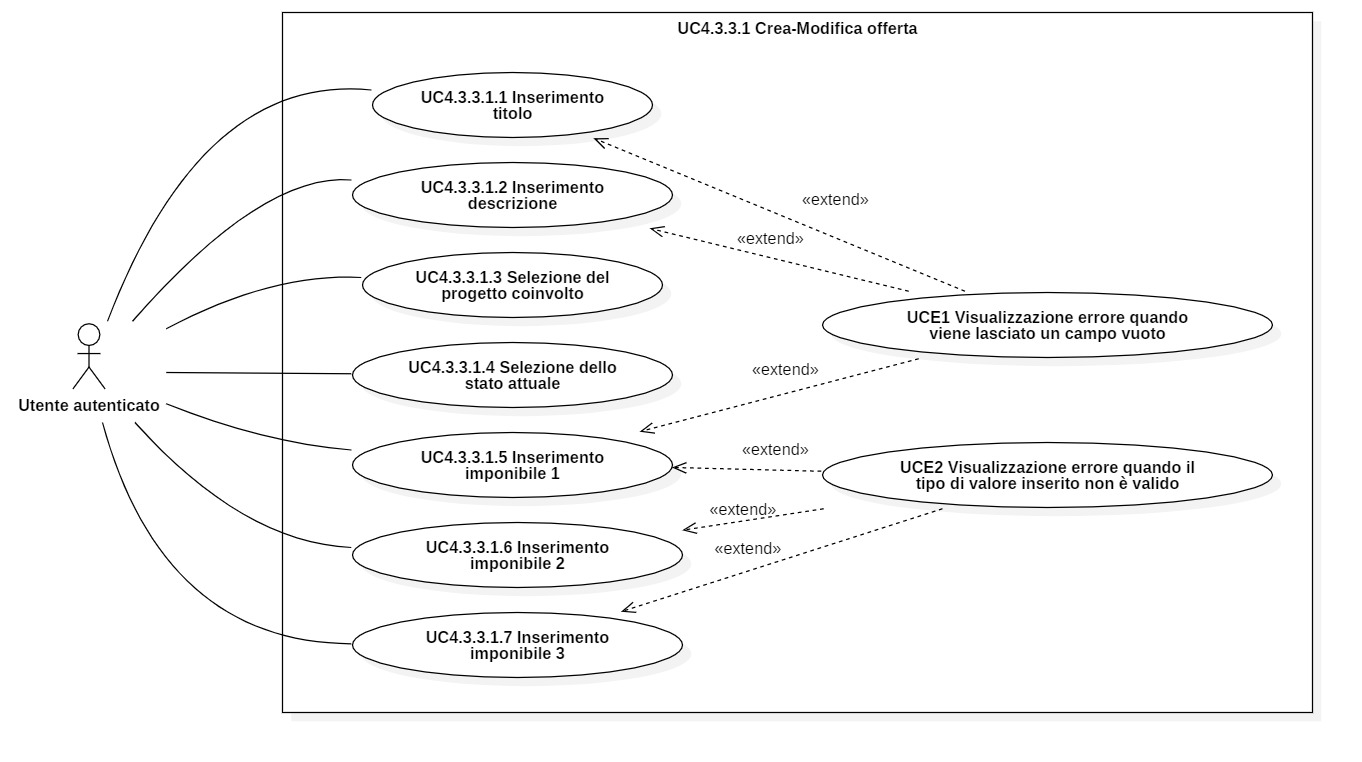
\includegraphics[width=400px]{../images/UC/.jpeg/UC4.3.3.1-nuovaModificaOfferta.jpg}
\caption{UC4.3.3.1: Crea-Modifica offerta}
\end{figure}

\begin{itemize}
\item \textbf{Attore primario}: Utente autenticato.
\item \textbf{Precondizione}: L'attore ha selezionato: 
\begin{itemize}
\item l'opzione \textit{nuova offerta} dal dettaglio di un cliente;
\item l'opzione \textit{modifica} dal dettaglio di un'offerta.
\end{itemize}
\item \textbf{Postcondizione}: L'attore ha creato/modificato un'offerta.
\item \textbf{Scenario principale}: 
\begin{enumerate}
\item L'attore inserisce/modifica il titolo di un'offerta [UC4.3.3.1.1].
\item L'attore inserisce/modifica la descrizione di un'offerta [UC4.3.3.1.2].
\item L'attore seleziona/modifica il progetto di riferimento di un'offerta [UC4.3.3.1.3].
\item L'attore seleziona/modifica lo stato attuale di un'offerta [UC4.3.3.1.4].
\item L'attore inserisce/modifica l'imponibile 1 di un'offerta [UC4.3.3.1.5].
\item L'attore inserisce/modifica l'imponibile 2 di un'offerta [UC4.3.3.1.6].
\item L'attore inserisce/modifica l'imponibile 3 di un'offerta [UC4.3.3.1.7].
\end{enumerate}
\item \textbf{Estensioni}: 
\begin{itemize}
\item L'attore visualizza un messaggio di errore quando viene lasciato un campo vuoto [UCE1].
\item L'attore visualizza un messaggio di errore quando viene inserito un tipo di valore non compatibile con quello del campo di interesse [UCE2].
\end{itemize} 
\end{itemize}

\pagebreak

\subsection{UC5: Tabella offerte}
\begin{figure}[!h]
\centering
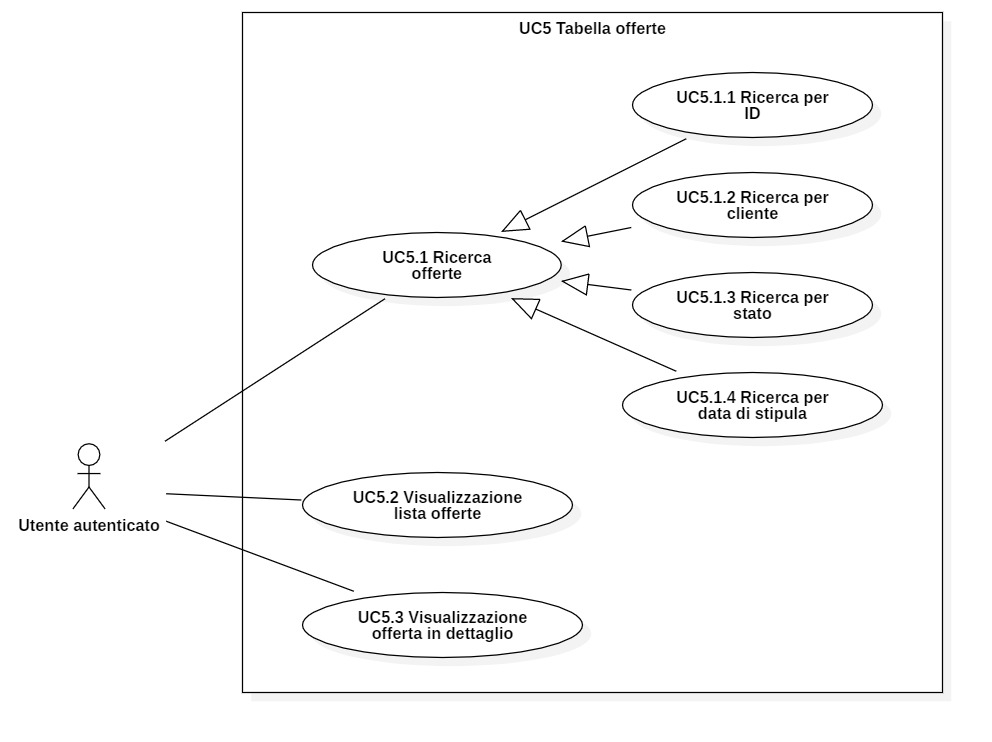
\includegraphics[width=400px]{../images/UC/.jpeg/UC5.0-tabellaOfferte.jpg}
\caption{UC5: Tabella offerte}
\end{figure}

\begin{itemize}
\item \textbf{Attore primario}: Utente autenticato.
\item \textbf{Precondizione}: L'attore ha selezionato l'opzione \textit{tabella offerte} dal menu.
\item \textbf{Postcondizione}: L'attore ha accesso alla tabella delle offerte.
\item \textbf{Scenario principale}: 
\begin{enumerate}
\item L'attore cerca una o più offerte tramite la funzionalità di ricerca [UC5.1].
\item L'attore visualizza la lista completa delle offerte presenti nel sistema [UC5.2].
\item L'attore visualizza un'offerta nel dettaglio [UC5.3].
\end{enumerate}
\item \textbf{Generalizzazioni}:
\begin{enumerate}
\item L'attore ricerca un'offerta per ID [UC5.1.1].
\item L'attore ricerca un'offerta per cliente associato [UC5.1.2].
\item L'attore ricerca un'offerta per stato attuale [UC5.1.3].
\item L'attore ricerca un'offerta per data di stipula [UC5.1.4].
\end{enumerate}
\end{itemize}

\pagebreak

\subsection{UC5.2: Visualizzazione lista offerte}
\begin{figure}[!h]
\centering
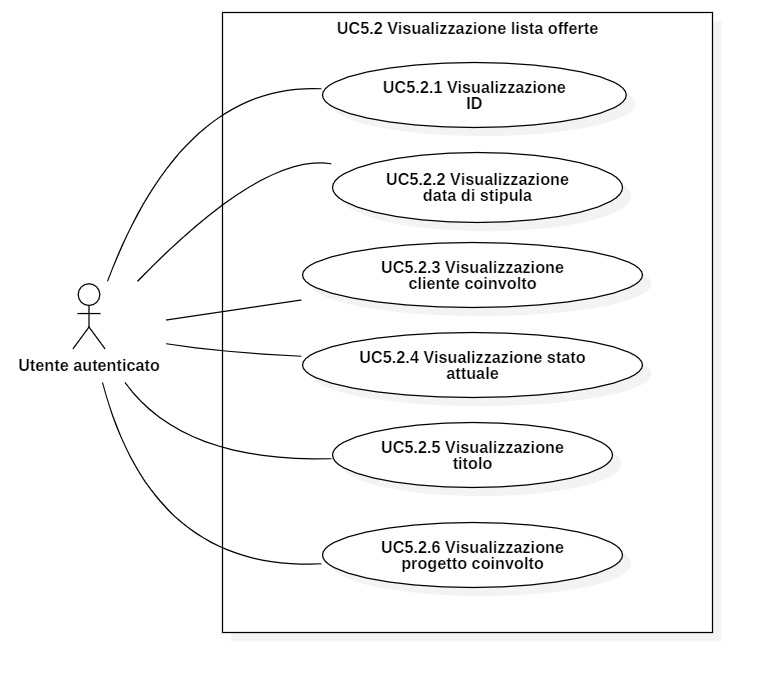
\includegraphics[width=300px]{../images/UC/.jpeg/UC5.2.0-visualizzazioneListaOfferte.jpg}
\caption{UC5.2: Visualizzazione lista offerte}
\end{figure}

\begin{itemize}
\item \textbf{Attore primario}: Utente autenticato.
\item \textbf{Precondizione}: L'attore ha accesso alla tabella delle offerte.
\item \textbf{Postcondizione}: L'attore ha visualizzato la lista delle offerte.
\item \textbf{Scenario principale}: 
\begin{enumerate}
\item L'attore visualizza l'ID dell'offerta [UC5.2.1].
\item L'attore visualizza la data di stipula dell'offerta [UC5.2.2].
\item L'attore visualizza il cliente coinvolto nell'offerta [UC5.2.3].
\item L'attore visualizza lo stato attuale dell'offerta [UC5.2.4].
\item L'attore visualizza il titolo dell'offerta [UC5.2.5].
\item L'attore visualizza il progetto coinvolto nell'offerta [UC5.2.6].
\end{enumerate}
\end{itemize}

\pagebreak

\subsection{UC5.3: Visualizzazione offerta in dettaglio}
\begin{figure}[!h]
\centering
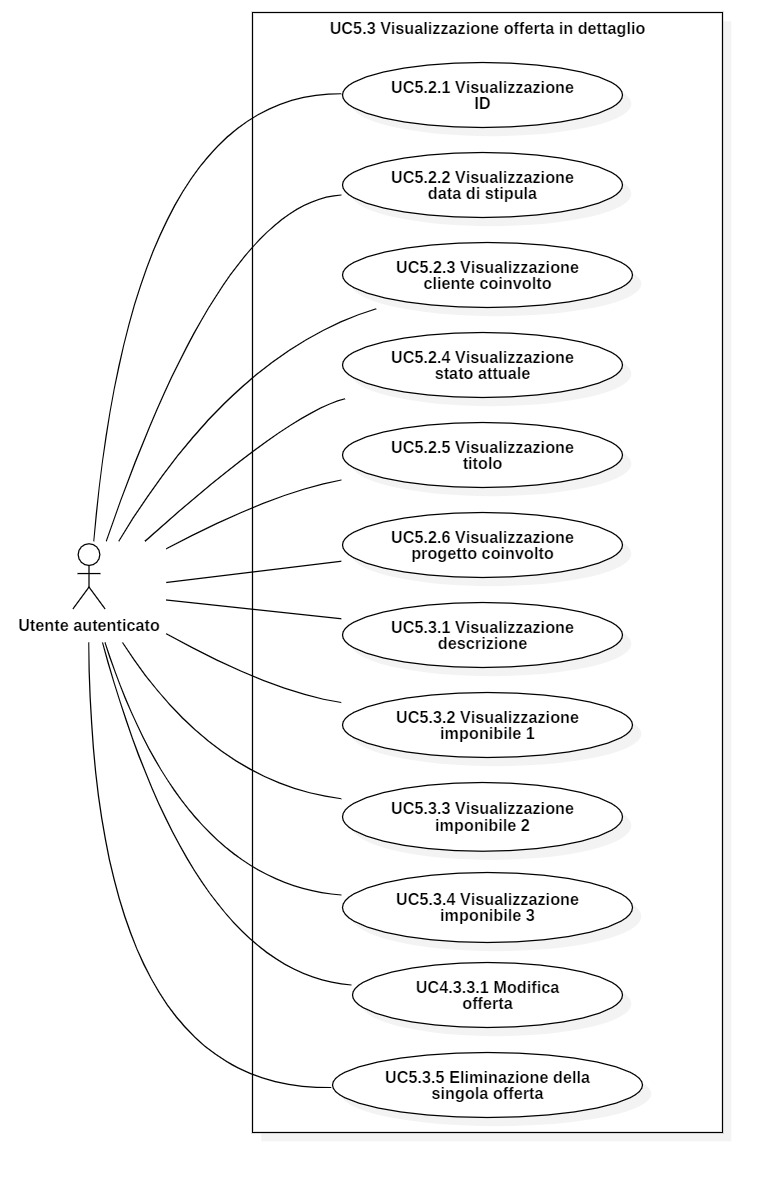
\includegraphics[width=300px]{../images/UC/.jpeg/UC5.3.0-visualizzazioneDettaglioOfferta.jpg}
\caption{UC5.3: Visualizzazione offerta in dettaglio}
\end{figure}

\begin{itemize}
\item \textbf{Attore primario}: Utente autenticato.
\item \textbf{Precondizione}: L'attore ha accesso alla tabella delle offerte.
\item \textbf{Postcondizione}: L'attore ha visualizzato il dettaglio di un'offerta.
\item \textbf{Scenario principale}: 
\begin{enumerate}
\item L'attore visualizza l'ID dell'offerta [UC5.2.1].
\item L'attore visualizza la data di stipula dell'offerta [UC5.2.2].
\item L'attore visualizza il cliente coinvolto nell'offerta [UC5.2.3].
\item L'attore visualizza lo stato attuale dell'offerta [UC5.2.4].
\item L'attore visualizza il titolo dell'offerta [UC5.2.5].
\item L'attore visualizza il progetto coinvolto nell'offerta [UC5.2.6].
\item L'attore visualizza la descrizione dell'offerta [UC5.3.1].
\item L'attore visualizza l'imponibile 1 dell'offerta [UC5.3.2].
\item L'attore visualizza l'imponibile 2 dell'offerta [UC5.3.3].
\item L'attore visualizza l'imponibile 3 dell'offerta [UC5.3.4].
\item L'attore può modificare l'offerta [UC4.3.3.1].
\item L'attore può eliminare l'offerta [UC5.3.5].
\end{enumerate}
\end{itemize}

\pagebreak

\section{Definizione e tracciamento dei requisiti}
Per concordare gli obiettivi da raggiungere e i problemi da risolvere sono stati trovati una serie di requisiti. 
Per identificare ciascun {\hyperref[sec:requisito-definition]{requisito}}\glsfirstoccur \; si è ricorso ad un codice identificativo composto \textbf{R [F/V] O N} dove:
\begin{itemize}
\item \textbf{R} = requisito;
\item \textbf{F} = funzionale;
\item \textbf{V} = di vincolo;
\item \textbf{O} = obbligatorio;
\item \textbf{N} = numero del requisito.
\end{itemize}

\noindent Di seguito si riporta una tabella contenente tutti i requisiti individuati con relativa descrizione e riferimento al relativo use case.

\pagebreak

\subsection{Requisiti funzionali}
\begin{table}[h!]
	\centering
	\begin{tblr}{
		colspec={|c|X|c|},
		row{odd}={bg=white},
		row{even}={bg=gray!30},
		row{1}={bg=white,fg=black}
		}
		\hline 
		\textbf{Identificativo} & \textbf{Descrizione} & \textbf{Use case} \\
		\hline
		 RFO1 &	L’utente deve poter utilizzare il menu. &	UC0\\
RFO2 &	L’utente deve poter creare un nuovo progetto. &	UC1\\
RFO3 &	L’utente deve poter accedere alla tabella dei progetti. &	UC2\\
RFO4 &	L’utente deve poter accedere alla tabella dei progetti aperti. &	UC3\\
RFO5 &	L’utente deve poter accedere alla tabella dei clienti. &	UC4\\
RFO6 &	L’utente deve poter accedere alla tabella delle offerte. &	UC5\\
RFO7 &	L’utente inserisce il codice del progetto. &	UC1.1\\
RFO8 &	L’utente inserisce il titolo del progetto. &	UC1.2\\
RFO9 &	L’utente inserisce la descrizione del progetto. &	UC1.3\\
RFO10 &	L’utente inserisce la data di inizio del progetto. &	UC1.4\\
RFO11 &	L’utente seleziona il cliente committente del progetto. &	UC1.5\\
RFO12 &	L’utente seleziona il responsabile interno del progetto. &	UC1.6\\
RFO13 &	L’utente seleziona lo stato di avanzamento del progetto. &	UC1.7\\
RFO14 &	L’utente inserisce i giorni di sviluppo previsti. &	UC1.8\\
RFO15 &	L’utente seleziona la percentuale di avanzamento del progetto. &	UC1.9\\
RFO16 &	L’utente visualizza un errore quando lascia vuoto il campo codice del progetto. &	UCE1\\
RFO17 &	L’utente visualizza un errore quando lascia vuoto il campo titolo del progetto. &	UCE1\\
RFO18 &	L’utente visualizza un errore quando lascia vuoto il campo descrizione del progetto. & UCE1\\
RFO19 &	L’utente visualizza un errore quando lascia vuoto il campo data di inizio del progetto. &	UCE1\\
RFO20 &	L’utente visualizza un errore quando lascia vuoto il campo giorni di sviluppo del progetto. &	UCE1\\
RFO21 &	L’utente può ricercare uno o più progetti. &	UC2.1\\
RFO22 &	L’utente ricerca un progetto per ID. &	UC2.1.1\\
RFO23 &	L’utente ricerca un progetto per cliente associato. &	UC2.1.2\\
RFO24 &	L’utente ricerca un progetto per responsabile interno. &	UC2.1.3\\
RFO25 &	L’utente ricerca un progetto per codice di progetto. &	UC2.1.4\\
RFO26 &	L’utente ricerca un progetto per titolo. &	UC2.1.5\\
		\hline
	\end{tblr}
\end{table}

\pagebreak

\begin{table}[h!]
	\centering
	\begin{tblr}{
		colspec={|c|X|c|},
		row{odd}={bg=white},
		row{even}={bg=gray!30},
		row{1}={bg=white,fg=black}
		}
		\hline 
		\textbf{Identificativo} & \textbf{Descrizione} & \textbf{Use case} \\
		\hline
		 RFO27 &	L’utente ricerca un progetto per stato di avanzamento. &	UC2.1.6\\
RFO28 &	L’utente ricerca un progetto per data di creazione. &	UC2.1.7\\
RFO29 &	L’utente visualizza la lista dei progetti.&	UC2.2\\
RFO30 &	L’utente visualizza il dettaglio di un progetto. &	UC2.3\\
RFO31 &	L’utente visualizza l’ID di un progetto. &	UC2.2.1\\
RFO32 &	L’utente visualizza la stringa “codice - titolo” di un progetto. &	UC2.2.2\\
RFO33 &	L’utente visualizza il committente di un progetto.&	UC2.2.3\\
RFO34 &	L’utente visualizza il responsabile interno di un progetto.&	UC2.2.4\\
RFO35 &	L’utente visualizza lo stato di avanzamento di un progetto.&	UC2.2.5\\
RFO36 &	L’utente visualizza la data di inizio di un progetto.&	UC2.2.6\\
RFO37 &	L’utente visualizza i giorni di sviluppo previsti di un progetto.&	UC2.2.7\\
RFO38 &	L’utente visualizza la descrizione del progetto.&	UC2.3.1\\
RFO39 &	L’utente visualizza la percentuale di avanzamento del progetto.&	UC2.3.2\\
RFO40 &	L’utente visualizza e gestisce i clienti del progetto.&	UC2.3.3\\
RFO41 &	L’utente modifica il progetto.&	UC1\\
RFO42 &	L’utente elimina il progetto.&	UC2.3.4\\
RFO43 &	L’utente ricerca uno o più clienti. &	UC4.1\\
RFO44 &	L’utente ricerca un cliente per ID. &	UC4.1.1\\
RFO45 &	L’utente ricerca un cliente per codice. &	UC4.1.2\\
RFO46 &	L’utente ricerca un cliente per descrizione. &	UC4.1.3\\
RFO47 &	L’utente visualizza la lista dei clienti. &	UC4.2\\
RFO48 &	L’utente visualizza il dettaglio di un cliente. &	UC4.3\\
RFO49 &	L’utente visualizza l’ID di un cliente. &	UC4.2.1\\
RFO50 &	L’utente visualizza la stringa “codice – descrizione” di un cliente. &	UC4.2.2\\
RFO51 &	L’utente visualizza partita iva del cliente. &	UC4.3.1\\
RFO52 &	L’utente visualizza il codice fiscale del cliente. &	UC4.3.2\\
RFO53 &	L’utente visualizza la lista dei progetti associati al cliente. &	UC2.2\\

		\hline
	\end{tblr}
\end{table}

\pagebreak

\begin{table}[h!]
	\centering
	\begin{tblr}{
		colspec={|c|X|c|},
		row{odd}={bg=white},
		row{even}={bg=gray!30},
		row{1}={bg=white,fg=black}
		}
		\hline 
		\textbf{Identificativo} & \textbf{Descrizione} & \textbf{Use case} \\
		\hline
RFO54 &	L’utente visualizza la lista delle offerte associate al cliente.  &	UC4.3.3\\
RFO55 &	L’utente crea una nuova offerta. &	UC4.3.3.1\\
RFO56 &	L’utente visualizza la lista delle offerte. &	UC5.2\\
RFO57 &	L’utente inserisce il titolo dell’offerta. &	UC4.3.3.1.1\\
RFO58 &	L’utente inserisce la descrizione dell’offerta. &	UC4.3.3.1.2\\
RFO59 &	L’utente seleziona il progetto coinvolto nell’offerta. &	UC4.3.3.1.3\\
RFO60 &	L’utente seleziona lo stato attuale dell’offerta. &	UC4.3.3.1.4\\
RFO61 &	L’utente inserisce l’imponibile 1 dell’offerta. &	UC4.3.3.1.5\\
RFO62 &	L’utente inserisce l’imponibile 2 dell’offerta. &	UC4.3.3.1.6\\
RFO63 &	L’utente inserisce l’imponibile 3 dell’offerta. &	UC4.3.3.1.7\\
RFO64 &	L’utente visualizza un errore quando lascia vuoto il campo titolo dell’offerta. &	UCE1\\
RFO65 &	L’utente visualizza un errore quando lascia vuoto il campo descrizione dell’offerta. &	UCE1\\
RFO66 &	L’utente visualizza un errore quando lascia vuoto il campo imponibile 1 dell’offerta. &	UCE1\\
RFO67 &	L’utente visualizza un errore quando il tipo di valore inserito del campo imponibile 1 non è numerico. &	UCE2\\
RFO68 &	L’utente visualizza un errore quando il tipo di valore inserito del campo imponibile 2 non è numerico. &	UCE2\\
RFO69 &	L’utente visualizza un errore quando il tipo di valore inserito del campo imponibile 3 non è numerico. &	UCE2\\
RFO70 &	L’utente ricerca una o più offerte. &	UC5.1\\
RFO71 &	L’utente ricerca un’offerta per ID. &	UC5.1.1\\
RFO72 &	L’utente ricerca un’offerta per cliente associato. &	UC5.1.2\\
RFO73 &	L’utente ricerca un’offerta per stato attuale. &	UC5.1.3\\
RFO74 &	L’utente ricerca un’offerta per data di stipula. &	UC5.1.4\\
RFO75 &	L’utente visualizza il dettaglio di un’offerta. &	UC5.3\\
RFO76 &	L’utente visualizza l’ID di un’offerta. &	UC5.2.1\\
RFO77 &	L’utente visualizza la data di stipula di un’offerta. &	UC5.2.2\\
RFO78 &	L’utente visualizza il cliente coinvolto di un’offerta. &	UC5.2.3\\
RFO79 &	L’utente visualizza lo stato di un’offerta. &	UC5.2.4\\
		\hline
	\end{tblr}
\end{table}

\pagebreak

\begin{table}[h!]
	\centering
	\begin{tblr}{
		colspec={|c|X|c|},
		row{odd}={bg=white},
		row{even}={bg=gray!30},
		row{1}={bg=white,fg=black}
		}
		\hline 
		\textbf{Identificativo} & \textbf{Descrizione} & \textbf{Use case} \\
		\hline
RFO80 &	L’utente visualizza il titolo di un’offerta. &	UC5.2.5\\
RFO81 &	L’utente visualizza il progetto di un’offerta. &	UC5.2.6\\
RFO82 &	L’utente visualizza la descrizione dell’offerta. &	UC5.3.1\\
RFO83 &	L’utente visualizza l’imponibile 1 dell’offerta. &	UC5.3.2\\
RFO84 &	L’utente visualizza l’imponibile 2 dell’offerta. &	UC5.3.3\\
RFO85 &	L’utente visualizza l’imponibile 3 dell’offerta. &	UC5.3.4\\
RFO86 &	L’utente modifica l’offerta. &	UC4.3.3.1\\
RFO87 &	L’utente elimina l’offerta. &	UC5.3.5\\
		\hline
	\end{tblr}
	\setlength{\parskip}{3ex}
	\caption{Requisiti funzionali}
\end{table}

\subsection{Requisiti di vincolo}

\begin{table}[h!]
	\centering
	\begin{tblr}{
		colspec={|c|X|c|},
		row{odd}={bg=white},
		row{even}={bg=gray!30},
		row{1}={bg=white,fg=black}
		}
		\hline 
		\textbf{Identificativo} & \textbf{Descrizione}\\
		\hline
RVO1 & L'applicativo lato back-end è realizzato in Java.\\
RVO2 & L'applicativo lato back-end è realizzato mediante il framework Spring.\\
RVO3 & L'applicativo lato back-end è realizzato mediante il framework Hibernate.\\
RVO4 & L'applicativo lato fron-end è realizzato tramite HTML5, CSS3 e JavaScript\\
RVO5 & L'applicativo lato front-end è realizzato mediante il framework Bootstrap.\\
RVO6 & L'applicativo deve essere funzionante in tutte le sue componenti.\\
		\hline
	\end{tblr}
	\setlength{\parskip}{3ex}
	\caption{Requisiti di vincolo}
\end{table}